\documentclass[a4paper,12pt, answers]{exam} % answers
\usepackage[T1]{fontenc}
\usepackage{amsmath}
\usepackage{amssymb}
\usepackage{enumerate}
\usepackage{bm}
\usepackage{advdate}
\usepackage{datetime}
\usepackage{hyperref}
\usepackage[mathcal]{eucal}
\usepackage{dsfont}
\usepackage[numbered,framed]{matlab-prettifier}
\usepackage{graphicx}


\usepackage{url}
\newdate{issuedate}{15}{12}{2020}
\newdate{duedate}{29}{12}{2020}

% \newcommand{\duedate}[1][14]{%
% \begingroup
% \AdvanceDate[#1]%
% \today%
% \endgroup
% }%
%\input{lddef}
\usepackage[thehwcnt=5]{iidef}
\newcommand{\bx}{\bm{x}}    % x, vec
\newcommand{\bX}{\bm{X}}    % X, mat
\newcommand{\by}{\bm{y}}    % y, vec
\newcommand*{\defeq}{\stackrel{\text{def}}{=}}




\newcommand{\ut}{\underline{t}}    % t, vec

\newcommand{\bA}{\bm{A}}    % A, mat
\newcommand{\bn}{\bm{n}}    % n, mat

\newcommand{\bc}{\bm{c}}    % c, vec
\newcommand{\bu}{\bm{u}}    % u, vec
\newcommand{\bv}{\bm{v}}    % v, vec
\newcommand{\bw}{\bm{w}}    % w, vec
\newcommand{\bT}{\bm{T}}    % T, mat


\newcommand{\bY}{\bm{Y}}     % y, vec
\newcommand{\rvby}{\bm{\mathsf{y}}}    % y, rv. vec
\newcommand{\rvbx}{\bm{\mathsf{x}}}    % x, rv. vec
\newcommand{\bz}{\bm{z}}    % z, vec
% \newcommand{\bm}{\bm{m}}    % m, vec
\newcommand{\bt}{\bm{t}}    % t, vec
\newcommand{\bzero}{\bm{0}}    % 0, vec

\newcommand{\balpha}{\bm{\alpha}}    % alpha, vec
\newcommand{\bxi}{\bm{\xi}}    % xi, vec
\newcommand{\btheta}{\bm{\theta}}
\newcommand{\bTheta}{\bm{\Theta}}    % theta, vec
\newcommand{\bmu}{\bm{\mu}}    % mu, vec

\newcommand{\bSigma}{\bm{\Sigma}}    % Sigma, vec

\newcommand{\cL}{\mathcal{L}}  
\newcommand{\cX}{\mathcal{X}}  



\newcommand{\rvv}{\mathsf{v}}    % v, r.v.
\newcommand{\rvm}{\mathsf{m}}    % m, r.v.
\newcommand{\rvt}{\mathsf{t}}    % t, r.v.

\newcommand{\urvt}{\underline{\mathsf{t}}}    % t, r.v. vec

\newcommand{\T}{\mathrm{T}}    % transpose
\newcommand{\F}{\mathrm{F}}    % Frobenius
\newcommand{\BLS}{\mathrm{BLS}}    % BLS
\newcommand{\LLS}{\mathrm{LLS}}    % LLS
\newcommand{\MVU}{\mathrm{MVU}}    % MVU

\DeclareMathOperator*{\maximize}{maximize}    % maximize
\DeclareMathOperator*{\minimize}{minimize}    % minimize
\newcommand{\st}{\mathrm{subject~to}}    % minimize
\DeclareMathOperator{\tr}{Tr}
% \newcommand{\E}[1]{\mathbb{E}\left[{#1}\right]}
% \newcommand{\Prob}[1]{\mathbb{P}\left({#1}\right)}

\makeatletter
\@ifclasswith{exam}{answers}{\newcommand{\firstblock}{comments_ldps1}}{\newcommand{\firstblock}{policies}}
\makeatother
\thecourseinstitute{Tsinghua-Berkeley Shenzhen Institute}
\thecoursename{Learning From Data}
\theterm{Fall 2020}
\begin{document}

\pagestyle{headandfoot}
\runningheadrule


\newcounter{psctr}
\setcounter{psctr}{5} % set to the times of problem

\runningheader{Problem Set \thepsctr}
              {\textsc{Learning from Data}}
              { Page \thepage\ of \numpages}
\firstpagefooter{}{}{}
\runningfooter{}{}{}


\newcounter{Sequ}
\newenvironment{Sequation}
   {\stepcounter{Sequ}%
     \addtocounter{equation}{4}%
     \renewcommand\theequation{S\arabic{Sequ}}\equation}
   {\endequation}
%\mathrm{T}skip0pt

% \vspace*{\fill}
\centering

% \vspace{0.3em}
\centering
\renewcommand{\thequestion}{\arabic{psctr}.\arabic{question}}
	\hwname{Writing Assignment}
\courseheader

%\begin{center}
%  \underline{\bf Problem Set \thepsctr} \\
%\end{center}
\hwname{Problem Set}
\begin{flushleft}
  \textbf{Issued:} \displaydate{issuedate} \hfill
  \textbf{Due:} \displaydate{duedate} 
\end{flushleft}

\hrule 

\input{\firstblock}

%\pointname{}
%\vspace{\footskip}
\vspace{1em}


%\pointname{}
%\vspace{\footskip}
%\vspace{1em}

%\newpage\\
%Questions 4.1 \& 4.2 will help you understand some basic properties about maximal correlation and the alternating conditional expectation (ACE) algorithm.

\begin{questions}






\question[2] (Bellman equation and linear programming)
In a dynamic decision problem, given a policy $\pi$, the value function
satisfies the Bellman equation:
\begin{equation}\label{eq:bellman}
    V^{\pi}(s)
= R(s) + \gamma
\sum_{s' \in S}
P_{s\pi(a)}(s')V^{\pi}(s')
\end{equation}
Now we play a simple game in a 3x3 block square. Our goal is to move the red object from
the upper left $(0, 0)$ to the bottom right corner $(2,2)$ (See Figure \ref{fig:my_label}).
\begin{figure}[!ht]
    \centering
    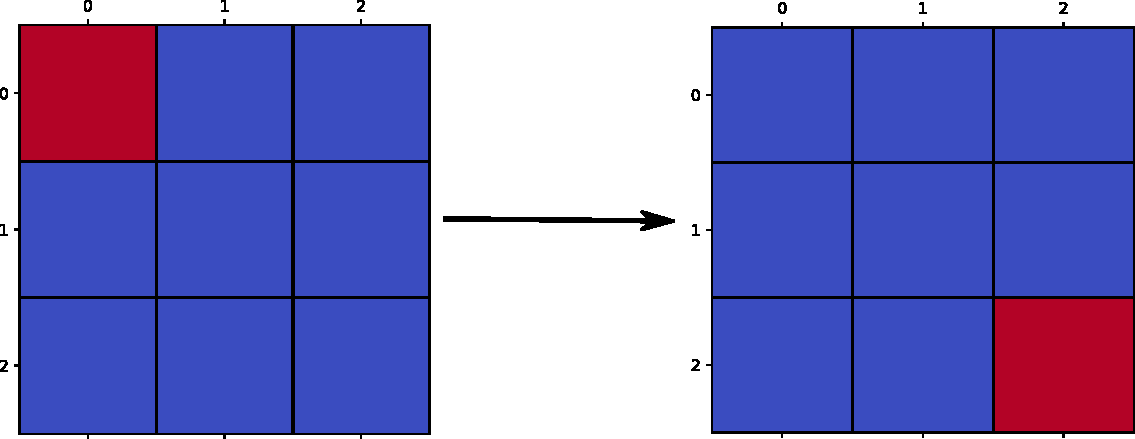
\includegraphics[width=0.7\textwidth]{Zeichnung.pdf}
    \caption{Moving a red object from upper left to bottom right}
    \label{fig:my_label}
\end{figure}
The state $s$ is represented by
a tuple $(x,y)$ where $x,y \in \{0, 1, 2\}$.
Choosing $\gamma=0.8$. The reward matrix satisfies $R((2,2))=1$ and $R(s)=0$ for other state $s$. 
There are four actions possible for each state
$\mathcal{A} = \{\textsf{up},\textsf{down},\textsf{left},\textsf{right}\}$, which deterministically cause the corresponding state transitions, except that actions that would take the agent off the grid in fact leave the state unchanged. For example $P_{s=(1,1), a=\textsf{right}}(s'=(1,2))=1$ and $P_{s=(1,1), a=\textsf{right}}(s'=(0,2))=0$.
Suppose $\pi$ is such a policy defined by
\begin{align*}
    \pi((i,j))= \begin{cases} (i+1,j) & i < 2 \\
    (i, j+1) & i = 2, j < 2 \\
    (2,2) & i=2 \textrm { and } j = 2
    \end{cases}
\end{align*}
Compute numerically the value function $V^{\pi}(s)$ for each $s$;
Make sure your computed $V^{\pi}(s)$
is the optimal value function, i.e. $V^{\pi}$ satisfy the condition
\begin{equation}
    V^*(s) = R(s) + \gamma\max_{a\in A}\sum_{s' \in S} P_{sa}(s')V^*(s')
\end{equation}

\begin{solution}

Let $p_{ij} = P(\pi((i,j)) = (i+1, j))$.
Applying the equation \eqref{eq:bellman} we have:
\begin{align*}
    V^{\pi}((2, 2)) & = 1 + 0.8 V^{\pi}((2,2)) \\
    V^{\pi}((2, 1)) & = 0.8 V^{\pi}((2,2)),\text{   }V^{\pi}((2, 0)) = 0.8 V^{\pi}((2,1)) \\
    V^{\pi}((1, 2)) & = 0.8 V^{\pi}((2,2)), \text{   } V^{\pi}((0, 2)) = 0.8 V^{\pi}((1,2)) \\
    V^{\pi}((1, 1)) & = 0.8 V^{\pi}((2, 1)), \text{   }
    V^{\pi}((0, 1)) = 0.8 V^{\pi}((1,1)) \\
    V^{\pi}((1, 0)) & = 0.8 V^{\pi}((2, 0)), \text{   }
    V^{\pi}((0, 0)) = 0.8 V^{\pi}((1, 0))\\
\end{align*}
Therefore, we can solve out:
\begin{equation}
    V^{\pi} = \begin{bmatrix}
    2.048 & 2.56 & 3.2 \\
    2.56 & 3.2 & 4 \\
    3.2 & 4 & 5
    \end{bmatrix}
\end{equation}

\end{solution}
\question[2] (Convergence of Value Iteration)
You have learned in class value iteration algorithm 
updates the value function
$V^{t+1}(s)=BV^{t}(s)$ for every state $s$,
where $B$ is the Bellman backup operator:
\begin{equation}
B\,V(s) = R(s) + \max_{a\in A} \gamma \sum_{s' \in S}
P_{sa}(s')V(s')
\end{equation}
\begin{parts}
\part[1] Show that Bellman backup operator is a contraction
operator.
That is, for any value function $V_1, V_2$,
\begin{equation}\label{eq:BV}
    \max_{s\in S}|B\,V_1(s) - B\, V_2(s)|
    \leq \gamma \max_{s\in S}|V_1(s) - V_2(s)|
\end{equation}
\part[1]  Assuming $R_{\max} = \max_{s \in S} R(s)$ and $V^{0}(s)=0$ for all $s \in S$,
show that
\begin{equation}\label{eq:vc}
    \max_{s\in S}|V^{t}(s) - V^*(s)| \leq \frac{\gamma^t R_{\max}}{1-\gamma}
\end{equation}
From \eqref{eq:vc}, we can see that $V^{t}(s)$ converges to $V^*(s)$.
\end{parts}
\begin{solution}
    \begin{parts}
    \part Using the definition of Bellman backup operator,
    \begin{align*}
       B\,V_1(s) - B\, V_2(s) &=
       \gamma(\max_{a\in A}\sum_{s' \in S}P_{sa}(s')V_1(s')-\max_{a\in A}\sum_{s' \in S}P_{sa}(s')V_2(s')) \\
       & \leq \gamma \max_{a\in A}\sum_{s' \in S}P_{sa}(s')
       (V_1(s') - V_2(s')) \\
       & \leq \gamma \max_{s\in S} |V_1(s) - V_2(s)|
    \end{align*}
    Similarly $B\,V_2(s) - B\, V_1(s)\leq \gamma \max_{s\in S} |V_1(s) - V_2(s)|$. Therefore
    $|B\,V_2(s) - B\, V_1(s)|\leq \gamma \max_{s\in S} |V_1(s) - V_2(s)|$. Taking the maximum on the left hand side we can show \eqref{eq:BV}.
    \part For $V^*$ we have $B\,V^*(s) = V^*(s)$ using
    \eqref{eq:BV} we have
    \begin{equation}
        \max_{s\in S}|V^{t+1}(s) -V^*(s)|\leq \gamma\max_{s\in S}
        |V^t(s) - V^*(s)| \leq \gamma^{t} \max_{s\in S}V^*(s)
    \end{equation}
    From Bellman equation \eqref{eq:bellman},
    we have $V^*(s) \leq R_{\max} + \gamma \max_{s\in S}V^*(s)$.
    Taking the maximum on the left hand side we have
    $V^*(s) \leq \frac{R_{\max}}{1-\gamma}$. Therefore,
    \eqref{eq:vc} holds.
    \end{parts}
\end{solution}
\question[3] (Mean Square Error) We mentioned Bias-Variance Tradeoff in class. We define the MSE of $\hat{X}$, an estimator of $X$ as $\mathrm{MSE}(\hat{X})\triangleq\E[(\hat{X}-X)^2]$. The variance of $\hat{X}$ is defined as $\Var (\hat{X})\triangleq\E[(\hat{X}-\E[\hat{X}])^2]$ and the bias is defined as $\mathrm{Bias}(\hat{X})\triangleq\E[\hat{X}]-X$.
\begin{parts}
	\part[1] Please prove that
	\begin{equation*}
	\mathrm{MSE}(\hat{X})=\Var(\hat{X})+(\mathrm{Bias}(\hat{X}))^2
	\end{equation*}
	\part[2] Our data are added with an independent Gaussian noise, say, $X+N$, where $\E[N]=0$ and $\E[N^2]=\sigma^2$ and the estimator is $\hat{X}$. We define the empirical MSE as $\E[(\hat{X}-X-N)^2]$. Please prove that
	\begin{equation*}
	\E[(\hat{X}-X-N)^2]=\mathrm{MSE}(\hat{X})+\sigma^2
	\end{equation*}
	The equation tells us that the empirical error is a good estimation of the true error. Thus, we can minimize the empirical error in order to properly minimize the true error.
\end{parts}

\begin{solution}
	\begin{parts}
		\part
	\begin{equation*}
	\begin{aligned}
			\E[(\hat{X}-X)^2]&=\E[(\hat{X}-\E[\hat{X}]+\E[\hat{X}]-X)^2]\\
			&=\E[(\hat{X}-\E[\hat{X}])^2] +\E[(\E[\hat{X}]-X)^2]+2\E[(\hat{X}-\E[\hat{X}])(\E[\hat{X}]-X)]\\
			&=\Var(\hat{X})+(\mathrm{Bias}(\hat{X}))^2
	\end{aligned}
	\end{equation*}
	, since that the expectation is only about $\hat{X}$
    \begin{equation*}
     \E[(\hat{X}-\E[\hat{X}])(\E[\hat{X}]-X)]=(\E[\hat{X}]-\E[\hat{X}])(\E[\hat{X}]-X)=0
    \end{equation*}
    \part
    \begin{equation*}
    \begin{aligned}
    \E[(\hat{X}-X-N)^2]&=\E[(\hat{X}-X)^2]+\E[N^2]+2\E[(\hat{X}-X)N]\\
    &=\mathrm{MSE}(\hat{X})+\sigma^2+2\E[(\hat{X}-X)]\E[N]\\
    &=\mathrm{MSE}(\hat{X})+\sigma^2
    \end{aligned}
    \end{equation*}
	\end{parts}
\end{solution}
\question[3]Important inequalities in Learning Theory.
\begin{parts} 

\part[1.5] (Markov's Inequality) Let $X$ be a non-negative random variable, then for every positive constant  $a$, please show that
\begin{align*}
    P(X\geq a) \leq \frac{\mathbb{E}(X)}{a}
\end{align*}

\part[1.5] (Chebyshev's inequality)For random variable $X$, if its expected value $\mathbb{E}(X)$ and variance $Var(X)$ are both finite, for every positive constant $a$, please show that 
\begin{align*}
    P(|X-\mathbb{E}(X)|\geq a)\leq \frac{Var(X)}{a^2}
\end{align*}

\end{parts}




\end{questions}

		


\end{document}



%%% Local Variables:
%%% mode: latex
%%% TeX-master: t
%%% End:
%  LocalWords:  headandfoot covariance
